\chapter{Calcolabilit\`a}

Una macchina di Turing \`e una definizione formale di algoritmo. La tesi di Church e Turing afferma che tutto \`e calcolabile con una macchina di Turing (quindi algoritmicamente).

Una macchina a stati finiti \`e una semplificazione di una macchina di Turing, ed \`e la versione pi\`u semplice di una macchina (ossia un algortimo) con cui si pu\`o realizzare qualcosa di pratico.

Il concetto di calcolabilit\`a \`e strettamente legato al concetto di computazione. Si stabilisce una famiglia di algoritmi in grado di risolvere uno specifico problema, e questa famiglia di algoritmi ha un insieme di problemi (oltre a quello che l'ha individuata) che \`e in grado di risolvere. La famiglia di algoritmi \`e ``potenziabile'', in grado di risolvere pi\`u problemi, rilassandone le ``propriet\`a'' e costruendo macchine sempre pi\`u potenti, fino alla macchina di Turing.

\section{Macchine a stati finiti}

\begin{defn}[Macchina di Mealy]
Una macchina di Mealy \`e una sestupla $(A, B, Q, \delta, q_0, F)$.
\begin{enumerate}
    \item $A$ \`e l'alfabeto di input;
    \item $B$ \`e l'alfabeto di output;
    \item $Q$ \`e l'insieme degli stati;
    \item $\delta$ \`e una funzione $\delta : Q \times A \to Q \times B^{\star}$ (chiamata di solito di transizione, ma dando anche un output \`e meglio chiamarla solo funzione);
    \item $q_0$ \`e uno stato iniziale;
    \item $F$ \`e un insieme di stati finali (che \emph{accettano} l'input).
\end{enumerate}
\end{defn}
Sia $A$ un alfabeto finito, $A^{\star}$ \`e l'insieme di tutte le stringhe finite a caratteri in $A$. $\lambda$ \`e la stringa vuota. L'insieme $A^{+}$ \`e $A^{\star} \setminus \{ \lambda \}$.

Data una funzione $g : A^{\star} \to B^{\star}$, se $g$ si applica solo a un sottoinsieme proprio di $A^{\star}$, allora $g$ \`e una funzione parziale. Altrimenti, $g$ si dice ``totale'' (se si applica a tutte le stringhe in $A^{\star}$).

Nel caso della macchina di Mealy vediamo che, essendoci un insieme $F$ di stati finali, le stringhe accettate non sono necessariamente tutte. $g$ \`e la funzione di un automa.

Un automa a stati finiti \`e un modo molto limitato di far funzionare un algoritmo. Si legge infatti un carattere uno alla volta, senza un buffer, senza possibilit\`a di tornare indietro. \`E un algoritmo in tempo reale senza memoria.

\emph{Ma!} Qualche problema interessante \`e risolvibile con una macchina a stati finiti.

Una macchina a stati finiti lavora ``online'', non ha tutto l'input visibile contemporaneamente, ma elabora i dati uno alla volta.

Ogni problema pu\`o essere formalizzato come una funzione $g : A^{\star} \to B^{\star}$.

\begin{defn}[Algoritmo online]
Si dice \emph{online} un algoritmo \code{AL} che per ogni stringa input $S \in A^{\star}$ calcola $g(S)$ in modo tale che:
\begin{enumerate}
    \item \code{AL} legge $S$ da sinistra a destra;
    \item quando \code{AL} legge l'$i$-esimo carattere di $S$ pu\`o accedere solo all'informazione fornita dal prefisso di lunghezza $i$ di $S$ (i caratteri gi\`a letti).
\end{enumerate}
Queste sono in realt\`a solo condizioni necessarie a rendere un algoritmo meno potente della macchina di Turing, ma non sufficienti. Quando l'algoritmo arriva alla fine della stringa, infatti, pu\`o spostarsi avanti e indietro liberamente, vedendo tutta la stringa.
\end{defn}

Per avere una macchina pi\`u debole di una macchina di Turing, ma pi\`u veloce nell'affrontare certi problemi, l'algoritmo deve poter accedere solo agli ultimi $k$ caratteri prima dell'$i$-esimo carattere, quindi non vede tutto il prefisso ma i suoi ultimi $k$ caratteri. Questo si chiama \emph{algoritmo online a memoria limitata}, e pi\`u piccolo \`e il $k$ e migliori sono le prestazioni che pu\`o ottenere.

\begin{defn}[Algoritmo online a memoria limitata]
Un algoritmo online a memoria limitata pu\`o accedere, nel momento in cui legge il carattere $i$, solo al suffisso di lunghezza $k$ del prefisso di $S$ di lunghezza $i$.
\end{defn}

Una macchina di Mealy \`e un algoritmo online senza buffer.

Non abbiamo parlato di quanto la puntina pu\`o stare su un singolo carattere. Un algoritmo online \`e in tempo reale se il tempo di esecuzione impiegato su ogni carattere \`e costante.

\subsection{Dizionari e fattorizzazione}

Se prendiamo $A^{\star}$, e consideriamo la struttura algebrica $(A^{\star}, +)$ con l'operazione $+$ di concatenazione, abbiamo che se $s_1, s_2 \in A^{\star}$, allora $s_1 + s_2 = s_1 s_2 \in A^{\star}$, quindi il gruppo \`e chiuso rispetto all'operazione. L'operazione \`e anche associativa, infatti $s_1 + (s_2 + s_3) = (s_1 + s_2) + s_3 = s_1 s_2 s_3 \in A^{\star}$. Ha anche l'elemento neutro, ossia $\lambda$. Questa struttura algebrica \`e un monoide ``libero'', che cresce liberamente concatenando elementi dell'insieme $A$. L'insieme $A^{+}$, con l'operazione di concatenazione, ha solo l'applicazione associativa, quindi \`e un semigruppo.

Si pu\`o parlare di fattorizzazione anche con le stringhe. Si pu\`o prendere un particolare sottoinsieme di $A^{\star}$ e poi chiederci se si pu\`o fattorizzare una stringa con la fattorizzazione usando questi particolari elementi.

\begin{defn}[Dizionario]
$D$ \`e un dizionario contenente i caratteri dell'alfabeto e un insieme di cosiddetti fattori $f_i$ dove $f_i$ \`e un elemento di $A^+$ (ossia una stringa non vuota) per $i$ che va da $1$ a $k$.
\[
D = A \cup \{ f_i : f_i \in A^{+} , \, 1 \le i \le k \}
\]
Quel che si ottiene \`e che ogni stringa in $A^{\star}$ \`e fattorizzabile con elementi di $D$.
\end{defn}
Qualsiasi stringa $s \in A^{\star}$ si pu\`o fattorizzare come concatenazione di $s_1 s_2 \dots s_i \dots s_t$ tali che $s_i \in D$ per $1 \le i \le t$. Il fatto che l'alfabeto sia nel dizionario garantisce la fattorizzabilit\`a di ogni stringa.

Ci sono problemi in cui \`e necessario massimizzare o minimizzare i costi, costi calcolati in base all'input. La fattorizzazione suggerisce un problema di minimizzazione: usare il minor numero possibile di fattori. C'\`e sempre una fattorizzazione banale usando i caratteri dell'alfabeto, che corrisponde al problema banale della massimizzazione dei fattori. Un altro problema \`e trovare un $D$ minimale, contenente il minor numero di fattori, e in grado di minimizzare il numero di fattori per le stringhe. Questa si chiama ``fattorizzazione ottimale''.

Se vogliamo rappresentare questo problema di fattorizzazione con una funzione $g : A^{\star} \to B^{\star}$, $A^{\star}$ \`e l'insieme delle stringhe che vogliamo fattorizzare, ma $B^{\star}$ chi \`e?

Il problema della fattorizzazione \`e alla base della compressione dei file. Persino la macchina di Mealy \`e in grado di fattorizzare delle stringhe.

Possiamo ridurre la fattorizzazione a decidere dove mettere delle virgole per distinguere le sottostringhe, e quindi bastano due caratteri. Decidiamo ad esempio di mettere un 1 all'inizio di ogni fattore. Quindi $g : A^{\star} \to \{ 0,1 \}^{\star}$.

Esistono particolari tipi di funzioni che mappano tutto in $\{ 0, 1\}$. Non \`e il caso della fattorizzazione. Si chiamano problemi decisionali: si deve rispondere s\`i o no a una determinata questione. Tutta la teoria della calcolabilit\`a si basa su problemi decisionali.

Vediamo il problema del pattern matching. In input si ha una stringa $S \in A^{\star}$, e un fattore $f \in A^{\star}$ anche lui. Ci chiediamo, \`e $f$ un fattore di $S$? Ossia, \`e $f$ una sottostringa di $S$? Se fatto in forza brutta, il tempo diventa $O(\abs{S} \cdot \abs{f})$, ossia dell'ordine del prodotto delle lunghezze. \`E possibile scendere a $O(\abs{S})$, e addirittura farlo con una macchina a stati finiti.

$S \in A^{\star}$, con $A$ un alfabeto finito, e poi abbiamo una stringa $f \in A^{\star}$, e ci chiediamo se $f$ \`e una stringa di $S$, ossia se $f$ \`e un pattern di $S$, ossia se $f$ \`e un fattore di $S$. 

Abbiamo detto che una macchina a stati finiti \`e una sestupla $(A, B, Q, \delta, q_0, F)$, in cui $A$ e $B$ sono alfabeti (di input e di output), $Q$ \`e l'insieme degli stati, $\delta : (Q \times A) \to (Q \times B^{\star})$ \`e una funzione di transizione, $q_0$ \`e uno stato finale, e $F$ \`e l'insieme di stati che accettano la stringa di input.

La macchina a stati finiti \`e l'algoritmo pi\`u semplice in tempo reale.

Per questo problema particolare, non serve l'alfabeto di output, e anche la funzione $\delta$ si semplifica, e diventa una funzione $\delta : Q \times A \to Q$. La macchina ora \`e una quintupla $(A, Q, \delta, q_o, F)$. Se lo stato finale appartiene a $F$ diciamo s\`i, altrimenti diciamo no. Questa macchina riconosce i linguaggi regolari. Tutte le stringhe per cui diciamo ``s\`i'' formano un sottoinsieme di $A^{\star}$, e per definizione un qualsiasi sottoinsieme di $A^{\star}$ \`e un linguaggio.

Riconoscere linguaggi \`e il problema che ci interesser\`a una volta arrivati alla macchina di Turing. Studiare il potere computazionale di una macchina equivale a studiare la capacit\`a della macchina di riconoscere un linguaggio.

Con $A_T$ si indica l'alfabeto del nastro, o Tape Alphabet, ossia $A_T = A \cup \{ <, > \}$, ossia l'alfabeto $A$ unito ai simboli di inizio e fine stringa.

Per non perdere tempo, e non dover mai tornare indietro con la puntina, vogliamo trovare il pi\`u lungo suffisso del prefisso gi\`a letto della stringa input che \`e prefisso di $f$. 

Fissato $f$, $\forall S \in A^{\star}$ la macchina deve dire se $f$ \`e un fattore di $S$. La macchina a stati finiti si pu\`o usare perch\'e abbiamo fissato $f$ in anticipo, altrimenti servirebbe una macchina di Turing. Il linguaggio \`e quindi l'insieme delle stringhe che hanno $f$ come fattore.

$\abs{Q} = \abs{f} + 1$, perch\'e ogni stato della macchina deve dirci quanti caratteri di f abbiamo riconosciuto. Il $+1$ \`e per lo stato iniziale, in cui non si \`e riconosciuto ancora nessun carattere.
\[
Q = \{q_0, q_1, \ldots, q_{\abs{f}}\}
\]
Questo si pu\`o formalizzare con un grafo orientato, molto spesso ciclico. Ciascuno stato \`e un nodo. Abbiamo fissato l'alfabeto $A$ e l'insieme degli stati $Q$, lo stato $q_0$, e l'insieme $F$ degli stati in cui si accetta la stringa. $F$ in realt\`a \`e in realt\`a solo $F = \{ q_{\abs{f}} \}$ (un singleton, un insieme di un unico elemento).

Ci manca solo la funzione di transizione $\delta = Q \times A \to Q$. La transizione va fatta con la regola gi\`a detta: bisogna passare dallo stato in cui ci si trova, allo stato che corrisponde al pi\`u lungo suffisso del prefisso gi\`a letto della stringa input che \`e prefisso di $f$. Bruttissimo a dirsi. Esiste sempre uno stato che rispetta questa condizione.

Passiamo a problemi di ricerca in cui si vuole fattorizzare una stringa. A \`e un alfabeto finito, $S \in A^{\star}$, e abbiamo un dizionario $D = A \cup \{ f_i : f_i \in A^{+} con 1 \le i \le k \}$, con $\abs{D} = k + \abs{A}$. Un insieme di stringhe quindi \`e un dizionario se ci sono anche i caratteri dell'alfabeto nell'insieme. Vogliamo suddividere ogni stringa $S$ in sottostringhe tali per cui ogni sottostringa appartiene al dizionario $D$. La fattorizzazione banale \`e quella che usa tutti i caratteri dell'alfabeto, e il costo della fattorizzazione \`e la lunghezza della stringa. \`E il massimo costo. La fattorizzazione che ci interessa \`e quella minima, in cui il costo \`e minimo. Il problema della stringa minima richiede una macchina di Turing.

\begin{figure}
\centering
\begin{tikzpicture}[->,>=stealth',shorten >=1pt,auto,node distance=2.8cm,semithick]
  \node[initial,state] (in)          {$q_0$};
  \node[state] (a)    [right of=in]  {$q_1$};
  \node[state] (ab)   [right of=a]   {$q_2$};
  \node[state] (aba)  [right of=ab]  {$q_3$};
  \node[state,accepting] (abac) [right of=aba] {$q_4$};

  \path (in)    edge              node {a} (a)
        (a)     edge              node {b} (ab)
        (ab)    edge              node {a} (aba)
        (aba)   edge              node {c} (abac);
\end{tikzpicture}
\caption{Macchina a stati finiti che riconosce la stringa ``abac''.}
\end{figure}

Il problema di minimizzare il costo si riesce a fare online (ossia con macchine pi\`u deboli della macchina di Turing) solo sotto particolari condizioni dello stato del dizionario.

$S$ \`e la stringa di input, con $S \in A^{\star}$. Vogliamo fattorizzare online (leggendo da sinistra a destra) la stringa $S$, selezionando a ogni passo algoritmico (quello del ``main loop'') il pi\`u lungo fattore in $D$.

Consideriamo ad esempio $A = \{ a,b \}$ e $D = \{ a, b, aba, aa, bb, bba \}$. La stringa $S$ \`e $abbbaabbbaa$. Con la pi\`u lunga fattorizzazione possibile otteniamo $a,bb,b,aa,bb,b,aa$. Con una struttura dati intelligente del dizionari si pu\`o fare in tempo reale, o addirittura con una macchina a stati finiti. \`E una procedura che funziona bene in pratica. Non produce per\`o la fattorizzazione minima.

La concatenazione \`e un'operazione algebrica come tutte le altre, quindi si pu\`o applicare la potenza dell'operazione, e $a^n$ significa una sequenza di a concatenate n volte.

Consideriamo l'alfabeto $A = \{ a, b \}$ e il dizionario $D = \{ a, b, ba, bab, ba^n \}$, con la stringa $S = baba^{n}$, abbiamo che il pi\`u lungo fattore a sinistra \`e $bab$, e l'unica cosa che si pu\`o fare \`e questa:
\[
S = bab,a,a,a,a,\ldots,a,a,a
\]
Si hanno $n+1$ fattori, quando la fattorizzazione ottimale \`e $S = ba, ba^n$, con solo due fattori.

Vediamo la complessit\`a di questa analisi online. Se il dizionario \`e memorizzato in una tabella, per ogni posizione di $S$ bisogna controllare quale \`e il pi\`u lungo fattore in quel punto, e controllare ciascun fattore carattere a carattere, quindi il tempo \`e $O(\abs{S} \cdot \abs{D} \cdot L)$, con $L = \max_{f_i \in D} \{ f_i \}$.

Questo tempo molto lungo \`e dovuto al fatto che $D$ non \`e rappresentato in maniera molto furba. Si pu\`o rappresentare $D$ in maniera pi\`u intelligente, e avere un algoritmo $O(\abs{S})$. Bisogna passare da una struttura tabellare a una struttura ad albero. Come radice si mette la stringa vuota $\lambda$, al primo livello si mettono i caratteri dell'alfabeto. Ogni fattore \`e un cammino dalla radice a un nodo, in cui ogni arco \`e rappresentato da un carattere dell'alfabeto. Ad ogni nodo associamo 0 o 1 se il fattore rappresentato dal cammino dalla radice a quel nodo \`e o meno nel dizionario.

\begin{figure}
\centering
\begin{tikzpicture}[->,>=stealth',level/.style={sibling distance = 5cm/#1,
  level distance = 1.5cm}] 
\node[circle, draw] {$\lambda$}
    % layer 1
    child{ node[circle, draw] {1}
        % layer 2
        child[missing] {}
        child{ node[circle, draw] {1} 
            % layer 3
            child{ node[circle, draw] {0} 
                % layer 4
                child{ node[circle,draw] {1} edge from parent node [above left] {a}}
                child[missing] {}
                % end layer 4
            edge from parent node[above left] {a}
            } 
            child[missing] {}
            % end layer 3
        edge from parent node[above right] {b}
        }
        % end layer 2
    edge from parent node[above left] {a}
    }
    % layer 1
    child{ node[circle, draw] {1} 
        % layer 2
        child{ node[circle, draw] {0}
            % layer 3
            child{ node[circle, draw] {1} edge from parent node[above left] {a}}
            child{ node[circle, draw] {1} edge from parent node[above right] {b}}
            % end layer 3
        edge from parent node[above left] {a}
        }
        child[missing] {}
        % end layer 2
    edge from parent node[above right] {b}
    } 
    % end layer 1
    ; 
\end{tikzpicture}
\caption{\code{TRIE} per il dizionario $D = \{ a, b, abaa, baa, ab, bab \}$}
\end{figure}

\[
D = \{ a, b, abaa, baa, ab, bab \}
\]
Non ha senso avere una foglia con etichetta 0. I nodi interni possono avere etichetta 0.

L'algoritmo deve ricordare l'ultimo nodo in cui ha trovato un 1. 

Questo \`e un algoritmo in tempo reale, ma non una macchina a stati finiti.

Un dizionario \`e prefisso (suffisso) se tutti i prefissi (suffissi) di un fattore del dizionario sono fattori del dizionario. In un dizionario prefisso, l'albero che lo rappresenta non ha nodi con etichetta 0. Tutti i prefissi di ogni fattore sono fattori del dizionario. Con i dizionari suffissi \`e possibile che ci siano nodi con etichetta 0.

La propriet\`a che serve per garantire l'ottimalit\`a, ossia la scelta di un numero ottimale di fattori, \`e la propriet\`a suffissa del dizionario.

Riprendiamo il problema della fattorizzazione. Abbiamo una stringa $S \in A^{\star}$, e un dizionario $D = A \cup \{ f_i \in A^+ : 1 \le i \le k\}$. Ogni stringa \`e fattorizzabile. Vogliamo minimizzare il numero di fattori. La scelta greedy per questo problema \`e quella di scorrere la stringa da sinistra a destra scegliendo ogni volta la sottostringa pi\`u lunga. Non \`e la scelta ottimale.

Abbiamo visto che \`e possibile fattorizzare una stringa in tempo reale se $s$ si rappresenta con un albero (detto \code{TRIE}).

\begin{defn}[\code{TRIE}]
Un \code{TRIE} \`e un albero radicato nella stringa vuota $\lambda$, con tanti figli quanto \`e la cardinalit\`a dell'alfabeto $A$ (si dice che l'albero \`e $\abs{A}$-ario). I nodi dell'albero sono etichettati come 1 se il cammino dalla radice al nodo concatenando le lettere dell'alfabeto $A$ produce un fattore nel dizionario $D$.
\end{defn}

Con un dizionario suffisso un algoritmo online greedy trova sempre la fattorizzazione ottimale, perch\'e in ogni istante l'algoritmo \`e a destra di una scelta ottimale.

Un dizionario prefisso non aiuta con il greedy online, ma esiste un modo perch\'e sia comodo. Con i dizionari suffissi non esiste il problema di ``tornare indietro'', perch\'e all'interno del \code{TRIE} non ci saranno nodi con etichetta 0.

La macchina a stati finiti \`e possibile con qualunque dizionario, con un po' di lavoro in pi\`u.

Vediamo la macchina $M = (A, B, Q, \delta, q_0, F)$ a stati finiti nel caso in cui abbiamo un dizionario prefisso. La fattorizzazione in output \`e fatta mettendo un 1 all'inizio (al primo carattere) di ogni fattore. Quindi l'alfabeto di output \`e $\{ 0, 1\}$. Le stringhe sono tutte fattorizzabili, quindi l'insieme degli stati finali $F$ sar\`a uguale a $Q$ (l'insieme di tutti gli stati). $Q$ sar\`a l'insieme dei nodi del \code{TRIE}. $q_0$ \`e $\lambda$, la radice dell'albero.

% disegnare albero ???

Bisogna definire la funzione di transizione. $\delta : Q \times A \to Q \times B^{\star}$. Le transizioni della funzione $\delta$ sono rappresentate graficamente con un arco orientato dal padre al figlio. Ciascuna foglia con qualsiasi input torna agli opportuni figli della radice. Per ciascun nodo, la funzione deve essere definita per ogni carattere nell'alfabeto di input. L'output \`e solo nel momento in cui da un nodo o da una foglia si torna ai nodi del primo livello, e sar\`a una sequenza di 0 per ciascun nodo del cammino, e poi un 1. Tutte le altre transizioni daranno $\lambda$ in output.

Formalizziamo. Sia $v$ un nodo del \code{TRIE}, e $a \in A$ un carattere dell'alfabeto che non corrisponde a un arco uscente dal nodo $v$. $v$ rappresenta una stringa $f \in A^{\star}$. La stringa $fa$ non \`e rappresentata nel \code{TRIE}. Deve essere fattorizzata con la tecnica greedy online. $fa = f_1 f_2 \ldots f_k$ \`e la sua fattorizzazione greedy online. La fattorizzazione va fatta non rispetto a quanto letto prima di $a$, ma rispetto a quanto letto al momento in cui si legge $a$. La fattorizzazione quindi va fatta rispetto a $f$.

La fattorizzazione giusta \`e quella $f_1 f_2 \ldots f_i$ tale per cui i fattori $f_{i+1} \ldots f_k$ rappresenta un nodo $w$ del \code{TRIE}. $i$ deve essere il pi\`u piccolo intero per cui questo vale.

Stiamo facendo preprocessing, praticamente. Si crea il fattore pi\`u lungo, e non si pu\`o pi\`u avanzare. Se l'etichetta \`e 1, la fattorizzazione \`e proprio $f a$, e quindi si ritorna al nodo corrispondente ad $a$ al primo livello dell'albero. Ma se l'etichetta \`e 0, allora c'\`e una fattorizzazione con pi\`u fattori. Vogliamo andare quindi a un nodo che corrisponde al pi\`u piccolo prefisso fattorizzato per cui il suffisso corrispondente \`e un nodo dell'albero. Bisogna aver fattorizzato prima quest'ultima stringa $f$.

La macchina costruita in questo modo avanza \emph{sempre}, con qualsiasi tipo di dizionario. L'input viene letto una volta sola, facendo un preprocessing del dizionario. Garantiamo quindi una fattorizzazione greedy online, ma non una fattorizzazione minima.

La fattorizzazione greedy online non funziona bene su esempi artificiali, ma funziona bene con esempi reali. Con un dizionario ben costruito, adatto al testo in input, il risultato \`e comunque buono. L'esempio \`e un testo italiano e un dizionario italiano: i fattori che si trovano sono parole con un senso, e quindi \`e molto probabile che i fattori successivi siano ancora parole con un senso.

Il modo per garantire di avere una fattorizzazione ottimale \`e dimostrare che quando si stabilisce l'$i$-esimo fattore la fattorizzazione sia a destra dell'$i$-esimo fattore di una fattorizzazione ottimale.

L'$i$-esimo fattore si produce all'$(i + 1)$-esimo passo. Questo algoritmo si chiama semi-greedy.

Vediamo dello pseudocodice per questo algoritmo. La stringa in input \`e $x_1 \ldots x_n$.

\begin{algorithm}
\caption{Fattorizzazione semi-greedy online}
\begin{algorithmic}
\State $j \gets 0$
\State $i \gets 0$
\Repeat
    \For{$k = j + 1 \to i + 1$}
        \State $h(k) : x_k \ldots x_{h(k)}$ (il pi\`u grande fattore in poszione $k$)
        \State $k' : h(k')$ \`e massimo (il fattore che va pi\`u a destra)
    \EndFor
    \State $x_k \ldots x_{k' - 1}$ \`e selezionato come fattore
    \State $j \gets k'$
    \State $i \gets h(k')$ (dove finisce la scelta che porta pi\`u a destra)
\Until{end of string}
\end{algorithmic}
\end{algorithm}

Dalla prossima lezione lavoreremo offline. Avremo tutta la stringa a disposizione, e vogliamo capire come trovare offline, dato un qualsiasi dizionario, la fattorizzazione minima. Si trasforma la stringa in un grafo orientato aciclico con $v_{n+1}$ nodi (dove $\abs{S} = n$), in modo tale che il cammino minimo da $v_{1}$ a $v_{n+1}$ d\`a la fattorizzazione minima della stringa.

Questo ci d\`a anche il concetto di riduzione: un problema si pu\`o ridurre ad un altro problema.

\begin{defn}[Cammino minimo]
Un cammino minimo \`e un cammino con il minor numero di archi da un nodo $u$ a un nodo $v$.
\end{defn}

La strigna $S$ \`e composta dai caratteri $s_1 \ldots s_n EOF$, con il carattere $EOF$ a indicare la fine della stringa. Quindi $\abs{S} = n+1$.

Ciascuna posizione (o carattere) della stringa \`e associata a uno degli $n+1$ nodi. Nella generica posizione $s_j$ si controllano tutti i fattori del dizionario, e se un fattore $f_i$ corrisponde alla sottostringa di $S$ che parte da $j$ si mette un arco dal nodo $v_{j}$ al nodo $v_{j + \abs{f_i}}$.

In una generica posizione il tempo massimo per inserire un nodo, usando un \code{TRIE} per rappresentare il dizionario, \`e dato dalla lunghezza del massimo fattore. Quindi in totale \`e $O(n \cdot L)$, con $L$ a indicare la massima lunghezza dei fattori in $D$.

Partendo dalla posizione $j$, si scende nel \code{TRIE} sulla stringa, e si mette un arco ogni volta che si trova un nodo del \code{TRIE} con etichetta 1.

Il cammino minimo si costruisce in tempo lineare sul numero degli archi con la visita in ampiezza.

Dato un alfabeto $A$, e una stringa $S \in A^{\star}$, con $\abs{A} = \alpha$, se codifichiamo l'alfabeto in binario, un generico carattere $a \in A$ \`e espresso con $\intsup{\log_2 (\alpha)}$ bit. Quindi una stringa $S$ \`e espressa con $\abs{S} \cdot \intsup{\log_2 (\alpha)}$ bit.

Se per\`o prendiamo un dizionario $D$ ben costruito rispetto alla stringa $S$ in input, possiamo fattorizzare la stringa e sostituire ciascun fattore con un puntatore a un elemento del dizionario.

Quindi ciascun fattore pu\`o essere sostituito da $\intsup{\log_2 (k + \alpha)}$ bit, con $k + \alpha$ a indicare la cardinalit\`a del dizionario. Vale quanto segue:
\[
\intsup{\log_2 (k + \alpha)} << \abs{f_i} \intsup{\log_2 (\alpha)}
\]
Tipicamente i fattori sono molto grandi. E aumentare di 1 i bit usati per i puntatori al dizionario permette di raddoppiare gli elementi del dizionario.

Si parla di codice da lunghezza variabile a lunghezza fissa: i fattori hanno lunghezza variabile, e vengono sostituiti con codici a lunghezza fissa (i puntatori, lunghi quanto visto sopra).

Un altro approccio al problema della compressione \`e quello di pensare di passare da codici a lunghezza fissa a codici a lunghezza variabile. Si prende la stringa e ci si chiede se esiste un modo pi\`u ``furbo'' per codificare i bit in maniera diversa. Invece di dare a tutti i caratteri lo stesso numero di bit, c'\`e un modo di dare a parole diverse codici di lunghezza differente?

Una codifica binaria formalmente \`e una funzione $f : A \to \{ 0, 1 \}^{\star}$.

Un codice prefisso ha un senso opposto a quello di dizionario prefisso. In inglese si parla di solito di prefix-free code e di prefix-closed dictionary.

Prendiamo come $A = \{ a, b, c, d, e, f \}$. L'immagine dell'insieme $A$, con un codice a larghezza fissa, \`e:
\[
f(A) = \{ 000, 001, 010, 011, 100, 101 \}
\]
L'immagine non \`e proprio un dizionario: non contiene gli elementi dell'alfabeto, quindi \`e uno pseudo-dizionario.

Con un codice prefisso, ogni parola di codice (ossia ogni elemento dell'immagine $f(A)$) \`e tale che ogni suo prefisso non \`e una parola di codice. Quando le parole sono tutte della stessa lunghezza questo \`e banalmente verificato. Con (la maggior parte dei) codici non prefissi \`e quasi impossibile decodificare un messaggio.

Per la decodifica con un codice prefisso si usa, al solito, un \code{TRIE}.

\subsection{Codice di Huffmann}

Abbiamo un alfabeto $A = \{ a, b, c, d, e, f \}$, e una stringa $S \in A^{\star}$. Conosciamo le occorrenze delle lettere nella stringa:
\begin{align*}
o(a) &= 45 \\
o(b) &= 26 \\
o(c) &= 17 \\
o(d) &= 15 \\
o(e) &= 2 \\
o(f) &= 8
\end{align*}
La lunghezza della stringa quindi \`e $\abs{S} = 113$. Qual \`e il codice prefisso per l'alfabeto che ci d\`a la codifica pi\`u corta? Se usiamo 3 bit per i caratteri dell'alfabeto, con un codice prefisso a larghezza fissa, la codifica $C(S)$ ha lunghezza $\abs{C(S)} = 336$.

Ma noi vogliamo una codifica che minimizzi la lunghezza della stringa codificata. Diamo quindi parole di codice pi\`u corte ai caratteri che occorrono pi\`u frequentemente.

L'input dell'algoritmo di Huffmann \`e l'alfabeto e il numero di occorrenze di ciascun carattere.

Ciascun carattere \`e un nodo. Ai due nodi che pesano di meno si d\`a un padre, di peso pari alla somma dei pesi dei due nodi figli. Questi due nodi si sostituiscono con il nodo padre. E si va avanti cos\`i, finch\'e non resta che un nodo fra quelli da inserire, che sar\`a quindi la radice. Fatto l'albero, i figli a sinistra prendono 0, i figli a destra prendono 1. Ciascuna foglia (che corrisponde a un carattere) avr\`a associato il percorso (come sequenza di 0 e 1) dalla radice a lei. Quella sar\`a la parola di codice associata al carattere.

I numeri di bit necessari sono la sommatoria del peso delle foglie per il livello a cui si trovano.

Un albero molto sbilanciato \`e un buon albero di Huffmann.

Si pu\`o anche passare dall'alfabeto $A$ all'insieme $A^k$ delle stringhe di lunghezza $k$ a caratteri in $A$. Il procedimento di Huffmann si pu\`o applicare, invece che ai caratteri dell'alfabeto, alle stringhe di lunghezza $k$, e le frequenze sono quelle dei blocchi di lunghezza $k$.

Esistono anche codici da lunghezza variabile a lunghezza variabile. Si fattorizza, con un dizionario a lunghezza variabile, e poi si applica Huffmann alla stringa fattorizzata. I fattori diventano i caratteri di un alfabeto esteso, su cui si costruisce l'albero di Huffmann.

La macchina che si occupa della codifica \`e una macchina a stati finiti banalissima. Ha un solo stato, che accetta, e degli archi dallo stato allo stato stesso, associati ai caratteri della codifica, e che producono in output la codifica dei caratteri (ossia, l'arco di a produce in output $f(a)$).

Per la decodifica, l'albero si basa sul \code{TRIE} costruito a partire dal dizionario. Gli stati accettanti $F$ sono le foglie, $Q$ contiene tutti gli stati dell'albero, $q_0$ sono le foglie. La $\delta$ in output d\`a sempre la stringa vuota, tranne sulle foglie, dove restituisce il cammino fino alla foglia. Dalle foglie, con l'input si torna ai figli della radice.

Last note: una codifica da lunghezza variabile a lunghezza variabile ha bisogno di un grafo con pesi sugli archi, se si cerca di minimizzare la codifica. Serve trovare il cammino minimo pesato. 

\section{Macchine di Turing}

Nel contesto della teoria della calcolabilit\`a l'unica cosa che ci interessa \`e stabilire cosa \`e calcolabile e cosa no, con un determinato modello algoritmico. La macchina di Turing \`e il modello ``pi\`u forte''.

Nello studio della calcolabilit\`a ci si pu\`o limitare a problemi decisionali di riconoscimento dei linguaggi. Prendendo un problema $f : A^{\star} \to B^{\star}$ qualsiasi, questo si pu\`o ridurre a un problema $f : A^{\star} \to A^{\star}$ (visto che il linguaggio $B^{\star}$ si pu\`o codificare con un altro alfabeto $A$).

Ora, un problema di riconoscimento dei linguaggi (o problema decisionale) \`e un problema $g : A^{\star} \to \{ 0, 1 \}$.
\[
L = \{ x : x \in A^{\star} \land g(x) = 1 \}
\]
$L$ \`e un linguaggio in $A^{\star}$ ($L \subseteq A^{\star}$).

Tornando al problema qualsiasi, possiamo prendere una coppia $(x,y)$ tale che $x, y \in A^{\star}$ (ossia, $(x,y) \in A^{\star} \times A^{\star}$). Ma di nuovo, possiamo ricodificare la coppia $(x,y)$ come un elemento di $A^{\star}$ (codificando, ad esempio, parentesi e virgola in $A^{\star}$).

Considerando $A = \{ 0, 1 \}$, e quindi $A^{\star} = \{ 0, 1 \}^{\star}$, si pu\`o ricodificare 0 con $00$ e 1 con $01$, e la virgola con $11$ (visto che non ci saranno mai due 1 consecutivi in questa nuova codifica).

Con questa formulazione, partendo da $f : A^{\star} \to A^{\star}$, possiamo definire un linguaggio $L \in A^{\star}$ dove:
\[
L = \{ (x,y) : y = f(x) \land x, y \in A^{\star} \}
\]
\`E il linguaggio in cui le stringhe codificano coppie in cui il primo elemento \`e un elemento di $A^{\star}$, e il secondo elemento \`e l'elemento in cui la $f$ mappa il primo elemento. La coppia $(x,y) \notin L$ se $f(x)$ non \`e definito (nel caso in cui la funzione $f$ \`e parziale) o se $y \neq f(x)$.

Con una macchina di Turing, conoscendo questo linguaggio, si pu\`o calcolare il valore di $f(x)$. Data una $x$, si genera ogni possibile $y$ e si controlla se la coppia $(x,y)$ appartiene al linguaggio.

\begin{defn}[Macchina di Turing]
Una macchina di Turing (per riconoscere linguaggi) \`e una quintupla $M = (Q, \Sigma, \delta, q_0, F)$, dove:
\begin{itemize}
    \item $Q$ \`e l'insieme di stati
    \item $\Sigma$ \`e l'alfabeto di input
    \item a differenza delle macchine a stati finiti, in cui la funzione di transizione era $\delta : Q \times \Sigma_T \to Q$, adesso la funzione di transizione \`e:
    \[
    \delta : Q \times \Sigma_T \times \Sigma_T \to Q \times \{ -1, 0, 1 \} \times \Sigma_T \times \{ -1, 0, 1 \}
    \]
    dove $\Sigma_T = \Sigma \cup \{ < , > \}$, che sono i caratteri di inizio e fine input, l'input \`e la terna formata da uno stato, dal carattere sull'input tape e dal carattere sul work tape, e l'output della funzione di transizione \`e la quaterna formata da uno stato, da un movimento della puntita di input (indietro, nessuno o avanti), da un output da scrivere sul work tape, e da un movimento della puntina sul work tape (indietro, nessuno o avanti)
    \item $q_0$ \`e lo stato iniziale
    \item $F$ \`e l'insieme di stati che accettano l'input
\end{itemize}
\end{defn}

Spesso la macchina di Turing si formalizza in maniera facile, parlando di due nastri (input tape e work tape), una puntina bidirezionale e un registro interno di stato. Ad ogni passo, la macchina cambia stato, sposta o meno la puntina di input, scrive qualcosa sull'output (se non deve scrivere niente, scrive lo stesso carattere), e sposta o meno la puntina sul work tape.

Alcune cose sono ``di troppo'': non \`e necessario avere la bidirezionalit\`a sul nastro di input, basta averla sul nastro di lavoro. Si pu\`o anche evitare di avere due nastri, basta usarne uno solo, spostandosi secondo necessit\`a.

Ora, dato un alfabeto $A$, e l'insieme $A^{\star}$ delle stringhe finite a caratteri in $A$, la stessa macchina di Turing $(Q, A, \delta, q_0, F)$ si pu\`o codificare con stringhe di $A^{\star}$. Ossia, esiste uno schema di codifica $C((Q, A, \delta, q_0, F)) \to x \in A^{\star}$. Il fatto che la stringa che codifica una macchina di Turing sia \emph{finita}, vuol dire che l'insieme di tutte le macchine di Turing \`e un insime infinito numerabile. Remember: $Q$ \`e un insieme \emph{finito} di stati, $F$ ancor di pi\`u, e cos\`i $A$ e $\delta$.

\begin{defn}[Insieme numerabile]
Un insieme infinito $S$ \`e numerabile se (e solo se) esiste una corrispondenza biunivoca tra $S$ e $\naturals$.
\end{defn}
Quindi deve esistere una funzione $f : \naturals \to S$ tale che $\forall s \exists n \in \naturals$ tale che $f(s) = n$ e $f(s) = f(s') \implies s = s'$.

$\parts (\naturals)$ non \`e in corrispondenza biunivoca con $\naturals$. Rappresentiamo ogni insieme in $\parts (\naturals)$ con il suo vettore caratteristico, ossia con la stringa di 0 e di 1 per cui alla posizione $i$ c'\`e uno 0 se $i$ non \`e contenuto nel sottoinsieme. Mettendo in tabella tutti $i$ vettori caratteristici, prendiamo il vettore caratteristico che sta sulla diagonale e complementiamolo. Questo vettore non pu\`o essere nella tabella: se lo fosse, la diagonale l'avrebbe intercettato in una riga $j$, alla colonna $j$, ma il vettore alla riga $j$ ha quel valore complementato. Assurdo.

$A^{\star}$, con $A$ finito, \`e numerabile. $\parts (A^{\star})$ \`e l'insieme di tutti i linguaggi sull'alfabeto $A$, e non \`e numerabile. Basta ripetere il metodo della diagonale con $A^{\star}$.

Bisogna capire cosa vuol dire che una macchina di Turing \emph{accetta} un linguaggio. Abbiamo tre possibilit\`a, invece delle due della macchina a stati finiti:
\begin{itemize}
    \item la macchina si ferma e accetta la stringa
    \item la macchina si ferma e non accetta la stringa
    \item la macchina \emph{non} si ferma.
\end{itemize}

Nella macchina di Turing esistono degli stati $q \in Q$ che sono ``halt state'', o ``stati di fermata''. Per quegli stati la funzione $\delta$ non \`e definita, ossia $\forall (x,y) \in \Sigma_T \times \Sigma_T$ si ha che $\delta(q,x,y)$ non \`e definito. $\delta$ pu\`o essere una funzione parziale.

La macchina si pu\`o fermare anche se $\delta$ non \`e definita solo su alcuni input, ma in questi casi lo stato $q$ non \`e esattamente uno stato di fermata.

\begin{defn}
Data una macchina di Turing $M$, il linguaggio associato $L(M)$ \`e tale che $L(M) = \{ x : M $ accetta $ x \}$. Una stringa $x$ \`e accettata se $L$ si ferma in un \emph{halt state} $q$ appartenente a $F$.
\end{defn}

Non diciamo niente su cosa succede quando $x \notin L(M)$. Ci sono quindi due possibilit\`a: o $M$ si ferma su uno stato che non appartiene a $F$, o non si ferma mai.

Torniamo a $\parts (A^{\star})$, ossia all'insieme di tutti i linguaggi a caratteri in $A$. $\Lambda$ \`e l'insieme di tutti e soli i linguaggi tali che per ogni siffatto linguaggio $L$ esiste una macchina di Turing che lo riconosce. Sicuramente \`e vero che $\Lambda \subset \parts (A^{\star})$. Ma \`e un sottoinsieme proprio? Esiste qualcosa che \`e fuori da $\Lambda$, ma appartiene a $\parts(A^{\star})$?

Chiamando $C$ l'insieme delle codifiche delle macchine di Turing, vale che $C \subseteq A^{\star}$. \`E sicuramente numerabile. Quindi anche $\Lambda$ \`e un insieme infinito numerabile, e quindi \`e un sottoinsieme proprio di $\parts (A^{\star})$. Anzi, i linguaggi non accettati da macchine di Turing sono \emph{molti} di pi\`u di quelli accettati. I linguaggi privi di grammatica sono la maggioranza.

$\Lambda$ si indica con $\code{RE}$, o insieme dei linguaggi Ricorsivamente Enumerabili. Tutti i linguaggi sono enumerabili, ma questi sono linguaggi per cui esiste una procedura calcolabile, algoritmica e quindi ricorsiva che li enumera, ossia che fornisce tutti gli elementi del linguaggio uno alla volta.

\subsection{Quando la macchina non si ferma}

Abbiamo detto che un dizionario contiene dei fattori uniti ai caratteri dell'alfabeto. Uno pseudo-dizionario, invece, non contiene tutti i caratteri dell'alfabeto. Con uno pseudo-dizionario non siamo sicuri di riuscire a fattorizzare ogni stringa. Consideriamo due pseudo-dizionarii $D$ e $D'$:
\begin{align*}
D &= \{ f_i : 1 \le i \le k \} \\
D' &= \{ f'_i : 1 \le i \le k' \} 
\end{align*}
Possiamo avere una stringa $S \in A^{\star}$ tale per cui la stringa non \`e fattorizzabile da nessuno dei due dizionari, altre fattorizzabili solo da uno dei due, altre fattorizzabili da entrambi.

La domanda ora \`e: esiste una stringa fattorizzabile sia da $D$ che da $D'$? Questa domanda definisce un linguaggio. L'input \`e dato dai due dizionari, e da questa domanda.

Si prendono i fattori del dizionario e si compongono stringhe, cercandone una fattorizzabile con entrambi i dizionari. Se la stringa esiste, prima o poi la troviamo. Ma se non esiste, la macchina potrebbe non fermarsi mai. Ora, potrebbe esserci un algoritmo intelligente in grado di capire, semplicemente guardando i dizionari, se esiste o meno una tale stringa.

Per dimostrare che con alcuni dizionari la macchina non si ferma mai, bisogna usare la ``riduzione tra linguaggi'', ossia ridurre un problema di riconoscimento di linguaggio a \emph{un altro} problema di riconoscimento di linguaggio.

Esistono anche linguaggi dentro $\code{RE}$ per cui la macchina in alcuni casi non si ferma! Una cosa che gi\`a Turing dimostr\`o, usando il metodo della diagonale.

Se la macchina di Turing non si ferma, rifiuta l'input: l'input non appartiene al linguaggio.

\subsection{Problema della fermata}

Il problema della fermata serve a dimostrare che esistono linguaggi in $\Lambda$ per cui alcune stringhe non appartenenti al linguaggio date in input alla macchina di Turing (che riconosce quel linguaggio) portano la macchina a non fermarsi.

Viene naturale ora definire un sottoinsieme di $\code{RE}$, che chiameremo $\code{RIC}$, che \`e l'insieme dei linguaggi ricorsivi. Un linguaggio $L$ appartiene a $\code{RIC}$ se esiste una macchina di Turing che riconosce $L$ e si ferma su ogni input. Quindi si ferma su uno stato che non accetta anche su input che non appartengono al linguaggio. Il termine tecnico \`e che la macchina $M$ \emph{decide} $L$.

L'insieme dei linguaggi ricorsivi \`e detto anche ``insieme dei linguaggi decidibili''. L'insieme $\code{RIC}$ \`e un sottoinsieme proprio di $\code{RE}$.

La codifica di una macchina di Turing \`e il linguaggio che la macchina accetta. La indichiamo con $C(M)$. Il linguaggio ha caratteri in $\{0,1\}$, e quindi $C(M) \subseteq \{0,1\}^{\star}$. Questo linguaggio lo chiamiamo anche ``programma'', e lo indichiamo con $P$.

Come al solito, a partire da un alfabeto $A$, possiamo codificare i suoi caratteri in $\{0,1\}^{\star}$, codificando poi a loro volta gli $0$ in $00$ e gli $1$ in $01$, e i ``separatori'' ($\diamond$) in $11$.

Possiamo codificare anche la macchina $P$ in $\{0,1\}^{\star}$, il separatore $\diamond$ in $\{0,1\}^{\star}$, e l'input $x$ in $\{0,1\}^{\star}$.

Abbiamo una stringa $P \diamond x$, dove $\diamond$ \`e la prima occorrenza del pattern pi\`u a sinistra. $P$ \`e la codifica di una macchina di Turing che si ferma sull'input $x$. Ma questo \`e un linguaggio:
\[
L = \left\{ P \diamond x : P \text{ \`e la codifica di una macchina di Turing che si ferma su } x \right\}
\]
Ma questo \`e un linguaggio ricorsivamente enumerabile? S\`i. Serve un algoritmo simulatore: prende in input una macchina di Turing e la simula. Questa \`e tipicamente chiamata ``macchina di Turing universale''.

La macchina di Turing universale \`e una macchina di Turing che prende in input un algoritmo e lo simula.

Se la macchina di Turing universale prende in input un algoritmo $P$ che non si ferma sull'input $x$, neanche la macchina di Turing universale si ferma. Ma abbiamo schivato il problema: bisogna ancora dimostrare che esiste una macchina di Turing (ossia, un algoritmo $P$) che su certi input non si ferma. Se esiste, questa macchina non si ferma. Ma: esiste?

Turing ha usato la diagonalizzazione per dimostrare che un algoritmo del genere. Per formalizzare questa diagonalizzazione, per\`o, dobbiamo formalizzare una propriet\`a dei linguaggi ricorsivi.

Prendiamo un linguaggio $L \subseteq \{0,1\}^{\star}$, e un linguaggio complemento $\bar{L} = \{0,1\}^{\star} - L$.

Il linguaggio $\bar{L}$ \`e ricorsivo, perch\'e se il linguaggio $L$ \`e ricorsivo, la sua macchina si ferma quando non accetta l'input. Quindi, nella famosa quintupla che identifica la macchina di Turing che accetta $L$, avevamo un insieme $Q$ degli stati e un insieme di stati che accettano $F$. La macchina complemento avr\`a lo stesso insieme di stati, e l'insieme di stati che accettano uguale a $Q \setminus F$.

Riformuliamo il linguaggio accettato dalla macchina di Turing universale. Prendiamo un linguaggio diverso, su cui possiamo sempre formulare il problema della fermata:
\[
L' = \left\{ x : x \text{ \`e la codifica di una macchina che si ferma su } x \right\}
\]
No ok. Tiriamone fuori un altro ancora:
\[
L'' = \left\{ x : x \text{ \`e la codifica di una macchina che accetta } x \right\}
\]
\`E leggermente diverso: si ferma, non accetta. $L'$ potrebbe accettare o rifiutare $x$, quando si ferma, mentre $L''$ se si ferma lo accetta. Quindi $L'' \subseteq L'$.

Quello che dobbiamo far vedere, quindi, \`e che $L''$ \`e indecidibile. \`E ovviamente ricorsivamente enumerabile. Continuano ad esserci casi in cui la macchina non si ferma mai (nel caso in cui $x$ non accetta $x$).

L'obiettivo \`e dimostrare che $\code{RIC}$ \`e un sottoinsieme proprio di $\code{RE}$ ($\code{RIC}$ $\subset$ $\code{RE}$), dimostrando che $L''$ non \`e in $\code{RIC}$.

Data una macchina $M$ e un input per $M$, questa pu\`o fare una di tre cose:
\begin{enumerate}
    \item accettare l'input
    \item fermarsi e rifiutare l'input
    \item rifiutare l'input non fermandosi
\end{enumerate}
Questa macchina identifica un linguaggio $L(M)$, che per\`o \`e anche il linguaggio identificato dalla macchina $M'$. $M'$ simula $M$, e se $M$ accetta l'input, anche $M'$ si ferma e lo accetta, se invece $M$ rifiuta l'input, $M'$ \emph{non si ferma} (indipendentemente da quello che fa $M$).

Un linguaggio ricorsivo si dice anche \emph{decidibile}.

Ora, per dimostrare che il linguaggio $L''$ non \`e ricorsivo, dobbiamo prima estendere la codifica di una macchina a $\{0,1\}^{\star}$.

Consideriamo l'insieme $S \subseteq \{0,1\}^{\star}$, che \`e l'insieme delle codifiche di una qualsiasi macchina di Turing. Prendiamo una stringa $x \notin S$. Che macchina di Turing le associamo? La macchina che rifiuta tutto, ossia che accetta come linguaggio l'insieme vuoto. Ossia: $x \notin S$ \`e la codifica di una macchina $M(L)$ il cui linguaggio \`e $L = \emptyset$. Quindi la macchina o si ferma immediatamente in uno stato che non appartiene a $F$, o cicla all'infinito.

Il linguaggio $L''$ non cambia, anche se associamo ad $x \notin S$ una macchina che si ferma e rifiuta su qualsiasi input. Ma per essere previdenti, pensiamo gi\`a da adesso di associare a $x \notin S$ una macchina che \emph{non} si ferma su qualsiasi input.

Mettiamo su una tabella le codifiche di tutte le macchine di Turing, una codifica per riga. Tutto $\{ 0,1 \}^{\star}$ sar\`a rappresentato nella tabella. Per qualche riga $i, j$, varr\`a che $L(M_i) = L(M_j)$. Poi, associamo ciascuna stringa in $\{0, 1\}^{\star}$ alle colonne della tabella. Le colonne le interpretiamo come input.

Nella casella $i, j$ metteremo $1$ se la macchina $M_i$ accetta la stringa $x_j$, $0$ altrimenti. Dato che il linguaggio $L''$ \`e un linguaggio ricorsivamente enumerabile, da qualche parte nella tabella ci sar\`a la macchina $M(L'')$, che riconosce $L''$. Il vettore caratteristico di $L''$ sar\`a anche sulla diagonale: la macchina codificata dalla riga $x_i$ accetta o non accetta la colonna $x_i$.

Vogliamo dimostrare che $L''$ \`e indecidibile. La propriet\`a dei linguaggi ricorsivi (o decidibili) \`e che il loro insieme \`e chiuso rispetto al complemento. Se un linguaggio $L$ appartiene all'insieme dei linguaggi ricorsivi, anche il suo complemento $\bar{L} = \{0,1\}^{\star} - L$ appartiene all'insieme dei linguaggi ricorsivi.

Ripetiamo: il vettore caratteristico di $L''$ \`e sulla diagonale. Il vettore caratteristico di $\{0,1\}^{\star} - L''$ si ottiene complementando il vettore caratteristico sulla diagonale. Quindi $\{0,1\}^{\star} - L'' = \bar{L''}$ \`e il vettore caratteristico del complemento di $L''$.

Ma il vettore caratteristico di $\bar{L''}$ si distingue da tutte le righe della tabella, quindi non pu\`o appartenere alla tabella, quindi non \`e ricorsivamente enumerabile. Se $\bar{L''}$ non \`e ricorsivamente enumerabile, $L''$ non pu\`o appartenere all'insieme dei linguaggi ricorsivi, perch\'e se il complemento di un linguaggio non \`e ricorsivamente enumerabile, il linguaggio non \`e ricorsivo.

Ora torniamo all'insieme $L'$:
\[
L' = \left\{ x : x \text{ \`e la codifica di una macchina di Turing che si ferma su } x \right\}
\]
Ora, sulla tabella associamo a 1 alla casella $(i,j)$ il significato di ``$x_i$ si ferma su $x_j$'', e 0 il significato di ``$x_i$ non si ferma su $x_j$''. Per ogni macchina che si ferma quando rifiuta, si pu\`o ricavare una macchina che non si ferma quando rifiuta.

Anche se abbiamo cambiato il significato di 0 e di 1, i vettori caratteristici dei linguaggi ricorsivamente enumerabili ci sono ancora tutti. Di nuovo, prendendo la diagonale e facendo il complemento, vediamo che il complemento non appartiene alla tabella, e quindi neanche $L'$ \`e ricorsivo.

Con il linguaggio $L$ definito prima, non si potrebbe usare questo metodo della diagonale con una tabella simile. Sulle righe avremmo infatti la combo algoritmo $P$, separatore $\diamond$ e input $x$, e sulle colonne l'input $x$.

Noi per\`o sappiamo gi\`a il fatto che il linguaggio ``$x$ che si ferma su $x$'' \`e indecidibile, e sfruttiamo il concetto di riduzione fra linguaggi. Sapendo che $L'$ \`e indecidibile, possiamo dimostrare l'indecidibilit\`a di altri linguaggi riconducibili a $L'$. Vogliamo passare da $L'$ a $L$, per dimostrare l'indecidibilit\`a di $L$.

\begin{defn}[Riduzione fra linguaggi]
La riduzione fra linguaggi \`e una funzione $f : \{0,1\}^{\star} \to \{0,1\}^{\star}$ calcolabile (o computabile), ossia esiste un algoritmo (ossia, una macchina di Turing) che la calcola.
\end{defn}
Questa funzione $f$ \`e tale che $x \in L' \iff f(x) \in L$. Quindi gli elementi del linguaggio $L'$ vengono mappati in elementi del linguaggio $L$, e quelli che \emph{non} sono nel linguaggio $L'$ \emph{non} vengono mappati nel linguaggio $L$. Se vale questa propriet\`a, $f$ \`e una riduzione da $L'$ a $L$, e lo si denota con $L' \le L$.

Una riduzione dimostra che il linguaggio a cui si riduce ($L$) non \`e meno complesso del linguaggio ridotto ($L'$). Se $L'$ non \`e decidibile, allora $L$ non \`e decidibile.

Se $L$ fosse decidibile, dovrebbe valere, contraddicendo quanto dimostrato prima, che $L'$ non \`e decidibile. Perch\'e? Perch\'e l'esistenza di questa funzione implica l'esistenza di una macchina che si ferma sempre e decide $L'$. Dato un qualsiasi input $x$, per vedere se $x \in L'$, applichiamo la funzione $f$, troviamo $f(x)$, usando la macchina di Turing che abbiamo detto esistere, e vediamo se $f(x) \in L$. Stiamo assumendo $L$ decidibile, quindi $f(x) \in L$ sappiamo stabilirlo. La procedura illustrata \`e un algoritmo, quindi questa procedura \`e una macchina che decide $L'$! Contraddizione, che implica l'assurdo della decidibilit\`a di $L$, e quindi l'indecidibilit\`a di $L$.

Rimettiamo assieme gli elementi:
\begin{align*}
L &= \left\{ P \diamond x : P \text{ si ferma su } x \right\} \\
L' &= \left\{ x : x \text{ si ferma su } x \right\}
\end{align*}
Inoltre, sappiamo che $L'$ \`e indecidibile. La funzione $f$ deve essere tale che:
\[
f(x) \mapsto P \diamond x
\]
per un qualche $P$. Ossia, $x \in L' \iff P \diamond x \in L$.

Per fare questa riduzione, dobbiamo estendere lo schema di codifica di $L$ a tutte le stringhe, ossia fare in modo che $P$, qualunque stringa sia, rappresenti una macchina di Turing. Con il problema aggiunto del separatore. 

Consideriamo l'insieme $S \subseteq \{0,1\}^{\star}$ che \`e l'insieme delle codifiche. $P \in S$, ovviamente. Supponiamo che, considerando la stringa $P \diamond x$, $x \notin S$. Se fosse che $x \in S$, la funzione $f(x)$ mapperebbe $x$ in $x \diamond x$, ossia $x \in S \implies P = x$.

Ma, se $x \notin S$, dobbiamo assumere una convenzione, ossia che $x$ \`e la codifica della macchina rappresentata dal suo pi\`u lungo prefisso. Ovviamente, il pi\`u lungo prefisso \emph{che codifica una macchina}. Non avendo detto ``prefisso proprio'', quando $x \in S$ il prefisso di $x$ che rappresenta una macchina \`e proprio $x$.

Se invece $x \notin S$, avr\`a sicuramente un altro prefisso improprio, che \`e la stringa vuota $\lambda$. Per convenzione, $\lambda$ codifica la macchina che rifiuta qualunque input, ossia che ha come linguaggio associato l'insieme vuoto.

Quindi, $f(x)$ va in $P \diamond x$ dove $P$ \`e il pi\`u lungo prefisso di $x$ che codifica una macchina. Ora \`e evidente che $x \in L' \iff P \diamond x \in L$, e quindi abbiamo trovato la riduzione di $L$ a $L'$.

Ora vedremo che la classe dei complementi dei linguaggi ricorsivamente enumerabili \`e una classe a s\'e. Questa classe si chiama $\code{CO-RE}$. Non \`e \emph{assolutamente} uguale a $\bar{\code{RE}}$, che \`e il complemento dell'insieme. $\code{CO-RE}$ \`e l'insieme dei linguaggi il cui complemento \`e ricorsivamente enumerabile. Complemento \`e riferito \emph{ai singoli linguaggi}, non all'insieme.
\[
L \in \code{CO-RE} \iff \bar{L} \in \code{RE}
\]
Ovviamente, se $L \in \code{CO-RE}$ e $L \in \code{RE}$, allora $L \in \code{RIC}$. \`E un se e solo se, anche se andrebbe dimostrato.

Per dirlo in altri modi, un linguaggio $L$ \`e ricorsivo se e solo se sia $L$ che $\{0,1\}^{\star} - L$ \`e ricorsivamente enumerabile. Si pu\`o dire anche che il complemento di un linguaggio ricorsivamente enumerabile e indecidibile non \`e ricorsivamente enumerabile.

Quindi, alla fine, quello che viene fuori \`e che $\code{RIC} = \code{CO-RE} \cap \code{RE}$. Dimostriamo questa parte.

\begin{proof}
Se $L$ \`e ricorsivo, per definizione $L$ \`e ricorsivamente enumerabile e $\bar{L}$ \`e ricorsivamente enumerabile (sempre per definizione). Quindi $\code{RIC} \subseteq \code{CO-RE} \cap \code{RE}$.

Se invece $\bar{L} \in \code{CO-RE}$ e $L \in \code{RE}$, allora esistono due macchime $M$ e $M'$ che riconoscono rispettivamente $L$ e $\bar{L}$. Non \`e detto che le due macchine si fermino sempre, ma sicuramente $M$ si ferma se l'input $x \in L$, e $M'$ si ferma se l'input $x \in \bar{L}$.

Da queste due macchine possiamo ricavare una macchina $M''$ che si ferma sempre e decide $L$. La macchina $M''$ esegue prima una transizione di $M$ e poi una transizione di $M'$. Si dovr\`a fermare, prima o poi, poich\'e l'unione di $L$ e $\bar{L}$ d\`a tutto $\{0,1\}^{\star}$.
\end{proof}

Dato un linguaggio $L \in \code{RE}$ e non in $\code{RIC}$, la macchina che accetta $L$ pu\`o non fermarsi se rifiuta l'input, e quindi la macchina che accetta $\bar{L}$ pu\`o non fermarsi se accetta l'input. La macchina che accetta $\bar{L}$ simula la macchina che accetta $L$, e rifiuta l'input quando la macchina che accetta $L$ accetta l'input. Si dice che la macchina che accetta $\bar{L}$ simula e contraddice la macchina che accetta $L$.

Chiamiamo $M$ la macchina che accetta $L$, e $M'$ la macchina che accetta $\bar{L}$ (e che quindi simula e contraddice $M$). Dato $x \in L$, $M'$ si ferma e rifiuta. Dato $x \in \bar{L}$, ci sono due casi: o $M'$ si ferma e accetta, o $M'$ non si ferma.

Con la tabella realizzata prima si possono fare un bel po' di cose. Definiamo, ad esempio, il linguaggio:
\[
L' = \{ f(x) : x \text{ si ferma su } f(x) \}
\]
dove $f : \{0,1\}^{\star} \to \{0,1\}^{\star}$ \`e biunivoca. Bisogna dimostrare che $L'$ \`e indecidibile.

Prima di tutto, perch\'e $L'$ sia in $\code{RE}$, bisogna dire che la funzione deve essere biunivoca (come \`e) e che deve avere l'inverso calcolabile. Questo non \`e necessario per dimostrare l'indecidibilit\`a.

Cambiamo la tabella permutando sulle colonne. Al posto della colonna $x_i$ mettiamo la colonna $f(x_i)$. La diagonale ora \`e il vettore caratteristico di $L'$.

Dire che un linguaggio \`e indecidibile significa dire che il linguaggio non appartiene a \code{RIC}.

Per dimostrare la tabella bisogna mettere il vettore caratteristico del linguaggio sulla diagonale di una tabella che rappresenta i linguaggi ricorsivamente enumerabili. Il complemento della diagonale non sar\`a nella tabella, e quindi il linguaggio non sar\`a ricorsivo.

Sia $S \subseteq \{ 0, 1\}^{\star}$ tale che $x \in S \iff x$ \`e la codifica di una macchina di Turing secondo uno schema di codifica dato.

Sia $f$ una funzione calcolabile $f : \{0,1\}^{\star} \to \{0,1\}^{\star}$ tale che l'immagine di $f$ \`e $S$.

\begin{esercizio}
Consideriamo il linguaggio $L$ definito come:
\[
L = \{ x : f(x) \text{ si ferma su } x \}
\]
Bisogna dimostrare che $L \in \code{RE} \setminus \code{RIC}$. Il linguaggio $L$ \`e ricorsivamente enumerabile: la macchina di Turing che lo accetta calcola $f(x)$ e poi simula $f(x)$ con $x$ come input.
\end{esercizio}

Bisogna far vedere che il linguaggio \`e fuori dai ricorsivi. Sulle colonne mettiamo tutte le stringhe di $\{0,1\}^{\star}$. Sulle righe, in corrispondenza della colonna $i$, mettiamo $f(x_i)$. Sulla diagonale abbiamo il vettore caratteristico del linguaggio, quindi il linguaggio \`e indecidibile.

\chapter{Complessit\`a}

Consideriamo d'ora in avanti solo i linguaggi ricorsivi.

\section{Macchine non deterministiche}

\begin{defn}[Macchina di Turing non deterministica]
Una macchina di Turing l'abbiamo definita come una quintupla $(Q, \Sigma, \delta, q_0, F)$, con la funzione $\delta : Q \times \Sigma_T \times \Sigma_T \to Q \times \{-1,0,1\} \times \{-1,0,1\} \times \Sigma_T$.

Le macchine di Turing non deterministice sono leggermente differenti. Sono una quintupla $(Q, \Sigma, \Delta, q_0, F)$ in cui $\Delta$ non \`e una funzione ma una pi\`u generale relazione:
\[
\Delta \subseteq Q \times \Sigma_T \times \Sigma_T \times Q \times \{-1,0,1\} \times \{-1,0,1\} \times \Sigma_T
\]
Una macchina non deterministica associa pi\`u stati ad una singola transizione. Con una macchina non deterministica non c'\`e un'unica computazione, ma ci sono diverse computazioni distinte. C'\`e un albero di computazioni. Le foglie dell'albero delle computazioni sono la fine delle computazioni.
\end{defn}

Una macchina di Turing deterministica \`e potente tanto quanto una macchina di Turing non deterministica. Una macchina non deterministica pu\`o sempre essere simulata da una macchina deterministica. \`E sufficiente visitare l'albero della macchina non deterministica.

Nella macchina non deterministica le computazioni avvengono in simultanea.

Introduciamo ora l'insieme dei linguaggi che pu\`o essere riconosciuto da una macchina non deterministica in tempo polinomiale, che chiamiamo $\code{NP}$. Poi, introduciamo l'insieme $\code{P}$ dei linguaggi che possono essere riconosciuti in tempo polinomiale da una macchina \emph{deterministica}.

La congettura di Cook dice che $\code{P} \neq \code{NP}$.

Una macchina non deterministica pu\`o ricondurre il problema del vertex cover a un problema decisionale, del tipo stabilire se una data coppia $<G,k>$ \`e tale che esiste un vertex cover del grafo $G$ di al pi\`u $k$ nodi.

Verificare se un insieme \`e un vertex cover si pu\`o fare in tempo polinomiale.

Spesso non sappiamo se una macchina non deterministica riesce a dire no in tempo polinomiale. Se dice s\`i, lo dice in tempo polinomiale sicuramente. Se dice no, bisogna studiare tutte le soluzioni.

Si pu\`o pensare ad un insieme $\code{CO-NP}$, dei linguaggi per cui si pu\`o stabilire in tempo polinomiale se una stringa non appartiene al linguaggio, ma non si sa dire nulla altrimenti.

Non si sa se i linguaggi in $\code{P}$ sono esattamente l'intersezione fra $\code{NP}$ e $\code{CO-NP}$.

Diamo una nuova definizione di $\code{NP}$. Un linguaggio $L$ \`e $L \in \code{NP} \iff \exists$ un algoritmo $A$ deterministico e polinomiale con input due stringhe binarie e una costante $C$ tale che:
\[
L = \left\{ 
\begin{array}{l}
x \in \{0,1\}^{\star} : \exists \text{ un certificato } y \in \{0,1\}^{\star} \\
\text{ con } \abs{y} = O \left( \abs{x}^c \right) \text{ tale che } A (x, y) = 1 
\end{array}
\right\}
\]
La classe $\code{NP}$ corrisponde a verifica in tempo polinomiale della correttezza di una soluzione. La classe $\code{P}$ corrisponde alla creazione in tempo polinomiale di una soluzione (corretta).

La classe dei linguaggi $\code{NPC}$ ($\code{NP}$ completi), se $\code{P} \subset \code{NP}$, \`e necessariamente fuori da $\code{P}$.

Riprendiamo il concetto di riduzione fra linguaggi. $f : \{0,1\}^{\star} \to \{0,1\}^{\star}$ \`e una riduzione polinomiale da $L$ a $L'$ se $f$ \`e calcolabile in tempo polinomiale e $x \in L \iff f(x) \in L'$. Per indicare questo, si usa il simbolo $L \le_{\code{P}} L'$. Serve a indicare che se $L' \in \code{P}$, anche $L \in \code{P}$.

Un linguaggio $L$ \`e $\code{NP}$ completo ($L \in \code{NPC}$) se $L \in \code{NP}$ e se $\forall L' \in \code{NP}$ si ha che $L' \le_{\code{P}} L$ ($L'$ \`e riducibile in tempo polinomiale ad $L$).

Se $\code{P} \subset \code{NP}$ allora $L \in \code{NPC} \implies L \notin \code{P}$.

Infatti, $L \in \code{P} \implies \code{P} = \code{NP}$. Abbiamo detto che se $L' \le_{\code{P}} L$ e $L \in \code{P}$, allora $L' \in \code{P}$. Abbiamo anche detto che $L \in \code{NPC}$ se $\forall L' \in \code{NP}$ si ha $L' \le_{\code{P}} L$, e avremmo quindi che $\forall L' \in \code{NP}$, $L' \in \code{P}$.

Se $L \in \code{NPC}$, $L \le_{\code{P}} L'' \implies L''$ \`e $\code{NP}$ completo. Infatti, $\forall L'$, $L' \le_{\code{P}} L \le_{\code{P}} L'' \implies \forall L'$, $L' \le_{\code{P}} L''$. Che \`e la definizione di linguaggio $\code{NP}$ completo, e quindi $L'' \in \code{NPC}$.

\subsection{Riduzioni alla 3-soddisfacibilit\`a}

Un linguaggio $\code{NPC}$ \`e il linguaggio dei circuiti booleani combinatoriali soddisfacibili. Un circuito $C$ \`e:
\[
C = \underbrace{x_1 x_2 \ldots x_n}_{\text{input}} \underbrace{c_1 c_2 \ldots c_m}_{\text{porte}}
\]
Dove $c_i =$ \code{OR}, \code{NOT} o \code{AND}, con $1 \le i \le m$. Un circuito si pu\`o rappresentare con una stringa binaria. $C'$\`e un linguaggio $L$, quindi, in $\{0,1\}^{\star}$ delle stringhe $C$ tali che $C$ \`e soddisfacibile.
\[
L = \{ < C > : C \text{ \`e soddisfacibile} \}
\]
Supponendo che l'ordinamento delle porte logiche sia topologico, l'output \`e $c_m$. Ora, qualsiasi linguaggio in $\code{NP}$ si pu\`o ridurre al linguaggio dei circuiti soddisfacibili, usando questa definizione:
\[
L' \in \code{NP} \iff 
L' = \left\{ 
\begin{array}{l}
x \in \{0,1\}^{\star} : \exists \text{ un certificato } y \in \{0,1\}^{\star} \\
\text{ con } \abs{y} = O \left( \abs{x}^c \right) \text{ tale che } A (x, y) = 1 
\end{array}
\right\}
\]
Ora, dobbiamo far vedere che per ogni $L' \in \code{NP}$, $L' \le_{\code{P}} L$. Prima per\`o verifichiamo che $L \in \code{NP}$. Il ``certificato'' $y$ \`e l'assegnazione di verit\`a delle variabili di input che soddisfano il circuito. Il numero di assegnazioni \`e esponenziale, ma verificare un'assegnazione richiede un tempo polinomiale. Bisogna far vedere che esiste un algoritmo $A$: \`e l'algoritmo che simula il circuito. Quindi, $L \in \code{NP}$.

Il linguaggi dei circuiti soddisfacibili \`e praticamente equivalente al linguaggio delle formule soddisfacibili: si pu\`o passare dall'uno all'altro in tempo polinomiale (lineare, anzi).

Si pu\`o passare da una formula qualsiasi a una formula in forma normale congiuntiva, ossia un \code{AND} di una serie di clausole, in cui ogni clausola \`e un \code{OR} di letterali (variabili affermate o negate), tramite una serie di passaggi algebrici.

Porte logiche a molti ingressi (e una uscita) si possono rappresentare come una ``cascata'' di porte con due ingressi ciascuna. 

Il problema di partenza, per la teoria della $\code{NP}$ completezza, \`e quello di trovare una formula booleana in forma normale congiuntiva in cui ogni clausola ha esattamente tre letterali. Si chiama \code{3-CNF}.

Sappiamo che se $L \le L'$ e $L$ \`e $\code{NP}$-completo, allora $L'$ \`e $\code{NP}$-completo.

Vediamo qualche problema sui grafi che \`e stato dimostrato essere $\code{NP}$-completo.

Consideriamo un grafo $G = (V,E)$. Vogliamo trovare il pi\`u grande sottografo completo di $G$. Un sottografo completo c'\`e sempre, nel caso estremo \`e un singolo nodo (considerando i singoli nodi adiacenti a s\'e stessi). Scriviamo la domanda come: esiste un sottografo completo di almeno $k$ nodi?

Abbiamo quindi un linguaggio dato dalle coppie $<G, k>$ per cui la risposta \`e \emph{S\`I}. Si pu\`o ridurre questo linguaggio al linguaggio della 3-soddisfacibilit\`a. Ma prima, bisogna dimostrare che \`e in $\code{NP}$.

Il certificato che dimostra l'appartenenza di questo linguaggio a $\code{NP}$ \`e il vettore caratteristico di $V(G)$ tale per cui tutti i nodi nel sottoinsieme sono collegati fra loro.

La macchina di Turing deterministica genererebbe tutti i sottoinsiemi di $V(G)$ e verificherebbe tutti questi sottoinsiemi finch\'e non trova un sottoinsieme di almeno $k$ nodi tutti collegati fra loro.
\[
\text{3-soddisfacibilit\`a } \le_{\code{P}} \text{ sottografo completo}
\]
Dobbiamo associare ad ogni coppia $<G, k>$ una formula booleana in forma normale congiuntiva in cui ogni clausola ha esattamente tre letterali.

Costruiamo il grafo: sar\`a un grafo $G(V,E)$ con $\abs{V} = 3 \, n$, associando a ogni nodo un letterale in una delle clausole di una formula con $n$ clausole.

Inseriamo un arco fra due nodi se i due nodi corrispondono a letterali di clausole diverse che non si contraddicono. Vuol dire che, dati due letterali $l^{i}_{j}$ e $l^{k}_{h}$ appartenenti alle clausole $i$ e $k$, vale che $i \neq k$ e $l^i_k \neq \bar {l^k_h}$.

Dire che la formula \`e soddisfacibile vuol dire affermare che per ogni clausola esiste un letterale vero, che vuol dire affermare che per ogni clausola esiste un letterale che non contraddice gli altri. I nodi associati a questi letterali formano un sottografo completo. Quindi considerando $<G,k>$, abbiamo che $k$ \`e $n$.

\begin{exmp}
Consideriamo questa formula:
\begin{align*}
& C_1 \land C_2 \land C_3 \\
C_1 &= x_1 \lor \bar{x_2} \lor \bar{x_3} \\
C_2 &= \bar{x_1} \lor x_2 \lor x_3 \\
C_3 &= x_1 \lor x_2 \lor x_3 \\
\end{align*}
La cardinalit\`a dell'insieme dei vertici del grafo \`e $\abs{V} = 3 \cdot 3$. Ai fini del linguaggio $<G,k>$, $k = 3$.

\begin{figure}
\centering
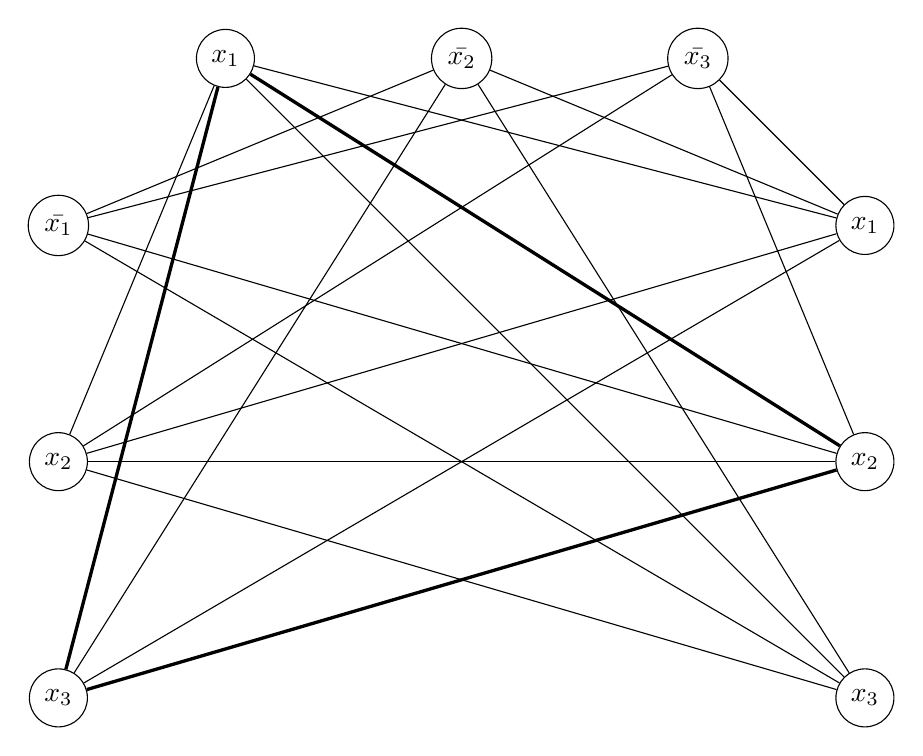
\begin{tikzpicture}[node distance = 3cm]
    \node (11) [circle, draw] {$x_1$};
    \node (12) [right of=11, circle, draw] {$\bar{x_2}$};
    \node (13) [right of=12, circle, draw] {$\bar{x_3}$};
    \node (21) [below left of=11, circle, draw] {$\bar{x_1}$};
    \node (22) [below of=21, circle, draw] {$x_2$};
    \node (23) [below of=22, circle, draw] {$x_3$};
    \node (31) [below right of=13, circle, draw] {$x_1$};
    \node (32) [below of=31, circle, draw] {$x_2$};
    \node (33) [below of=32, circle, draw] {$x_3$};

    \path [-] (11) edge (22) edge [very thick] (23) edge (31) edge [very thick] (32) edge (33)
              (12) edge (21) edge (23) edge (31) edge (33)
              (13) edge (21) edge (22) edge (31) edge (32)
              (21) edge (32) edge (33)
              (22) edge (31) edge (32) edge (33)
              (23) edge (31) edge [very thick] (32);
\end{tikzpicture}
\caption{\label{fig:grafo_soddisf}Grafo schifo puzza}
\end{figure}

% 11 12 13
% 21 22 23
% 31 32 33
% archi fra:
% 11 - 22 23 31 32 33
% 12 - 21 23 31 33
% 13 - 21 22 31 32
% 21 - 12 13 32 33
% 22 - 11 13 31 32 33
% 23 - 11 12 31 32
% 31 - 11 12 13 22 23
% 32 - 11 13 21 22 23
% 33 - 11 12 21 22 23
% riducibili a:
% 11 - 22 23 31 32 33
% 12 - 21 23 31 33
% 13 - 21 22 31 32
% 21 - 32 33
% 22 - 31 32 33
% 23 - 31 32

La formula \`e soddisfacibile se e solo se esiste un sottografo completo di cardinalit\`a (almeno) 3. E ce ne sono un sacco (figura \ref{fig:grafo_soddisf}). Una possibile assegnazione di verit\`a che soddisfa la formula \`e $x_1 = 0$, $x_2 = 0$ e $x_3 = 1$.
\end{exmp}

\chapter{Esercizi}

\section{L'immancabile di settembre}

\begin{esercizio}
$L$ \`e un linguaggio ricorsivamente enumerabile, e il suo complemento $\bar{L}$ \`e ricorsivamente enumerabile. Dimostrare che $L$ \`e ricorsivo.
\end{esercizio}

Abbiamo la macchina $m$ che accetta $L$, e la macchina $m'$ che accetta $\bar{L}$.

$L$ \`e ricorsivo se esiste una macchina di Turing che si ferma su qualsiasi input. La macchina $M$ che si ferma sempre su $L$ simula a passi alterni $m$ e $m'$. Se $m$ si ferma e accetta, anche $M$ si ferma e accetta. Se $m'$ si ferma e accetta, $M$ si ferma e rifiuta.

\section{Il favorito di ottobre}

\begin{esercizio}
Abbiamo il linguaggio $L$:
\[
L = \{ x : f(x) \text{ si ferma su } x \}
\]
Dimostrare che $L \in \code{RE} \setminus \code{RIC}$. La funzione $f$ \`e calcolabile e biunivoca, eh.
\end{esercizio}

Prima di tutto bisogna dimostrare che $L \in \code{RE}$. Prendiamo la macchina di Turing che calcola $f(x)$ e poi simula $f(x)$ con $x$ come input.

Poi, costruiamo una tabella con come colonne gli input $x_i$, e come righe le immagini $f(x_i)$. Mettiamo 1 alla casella $(i,j)$ se $f(x_i)$ si ferma su $x_j$, 0 altrimenti. Dato che $L$ \`e ricorsivamente enumerabile, da qualche parte nella tabella ci sar\`a la macchina che accetta $L$, codificata da una $f(x_k)$. Per come abbiamo costruito la tabella il vettore caratteristico di $L$, oltre ad essere alla riga di $f(x_k)$, sar\`a anche sulla diagonale.

Il complemento del vettore sulla diagonale non pu\`o essere nella tabella, quindi $\bar{L} \notin \code{RE}$, e quindi $L \notin \code{RIC}$.

\section{Il regalone di Natale}

\begin{esercizio}
Dimostrare l'esistenza di un linguaggio $L$ tale che n\'e $L$, n\'e il suo complemento $\bar{L}$ sono ricorsivamente enumerabili. 
\end{esercizio}

L'insieme di tutti i linguaggi \`e $\parts \left( A^{\star} \right)$, che non \`e un insieme numerabile. $\code{RE}$ \`e un insieme numerabile, cos\`i come $\code{CO-RE}$, e come la loro unione. Infatti ciascun linguaggio in $\code{RE}$ \`e individuato da (almeno) una macchina di Turing, e sappiamo che l'insieme delle macchine di Turing \`e numerabile. Quindi, necessariamente, $\code{CO-RE} \cup \code{RE} \subset \parts \left( A^{\star} \right)$.

\section{La superstar dei migliori bar di Caracas}

\begin{esercizio}
Consideriamo il linguaggio:
\[
L = \{ x : \exists y \text{ con } \abs{y} \le c \text{ su cui } x \text{ si ferma entro } c \text{ transizioni} \}
\]
Dimostrare che il linguaggio $L$ \`e ricorsivo.
\end{esercizio}

$L$ \`e ricorsivo se esiste una macchina di Turing che decide sempre l'input. Data una qualunque stringa $x$ in input, la macchina che decide $x$ deve creare tutte le possibili stringhe $y$ di lunghezza minore di $c$, e simulare la macchina codificata dall'input $x$ su ciascuna di queste stringhe per al pi\`u $c$ passi. Se dopo $c$ passi la macchina simulata non si trova in uno stato in $F$, questa passa alla stringa $y$ successiva. Se, invece, la macchina simulata accetta una qualunque delle $y$, la macchina che decide $L$ accetta l'input $x$.

Se nessuna delle stringhe $y$ viene accettata dalla macchina simulata, la macchina che decide $L$ rifiuta l'input $x$.

Sicuramente la macchina che decide $L$ si ferma, perch\'e per ogni input $x$ deve prendere in analisi un numero finito di stringhe, e simulare l'input $x$ su ciascuna di queste per un numero finito di passi.


















































